% Options for packages loaded elsewhere
\PassOptionsToPackage{unicode}{hyperref}
\PassOptionsToPackage{hyphens}{url}
\PassOptionsToPackage{dvipsnames,svgnames,x11names}{xcolor}
\documentclass[
  11pt,
]{article}
\usepackage{xcolor}
\usepackage[margin=2.5cm]{geometry}
\usepackage{amsmath,amssymb}
\setcounter{secnumdepth}{-\maxdimen} % remove section numbering
\usepackage{iftex}
\ifPDFTeX
  \usepackage[T1]{fontenc}
  \usepackage[utf8]{inputenc}
  \usepackage{textcomp} % provide euro and other symbols
\else % if luatex or xetex
  \usepackage{unicode-math} % this also loads fontspec
  \defaultfontfeatures{Scale=MatchLowercase}
  \defaultfontfeatures[\rmfamily]{Ligatures=TeX,Scale=1}
\fi
\usepackage[]{charter}
\ifPDFTeX\else
  % xetex/luatex font selection
\fi
% Use upquote if available, for straight quotes in verbatim environments
\IfFileExists{upquote.sty}{\usepackage{upquote}}{}
\IfFileExists{microtype.sty}{% use microtype if available
  \usepackage[]{microtype}
  \UseMicrotypeSet[protrusion]{basicmath} % disable protrusion for tt fonts
}{}
\makeatletter
\@ifundefined{KOMAClassName}{% if non-KOMA class
  \IfFileExists{parskip.sty}{%
    \usepackage{parskip}
  }{% else
    \setlength{\parindent}{0pt}
    \setlength{\parskip}{6pt plus 2pt minus 1pt}}
}{% if KOMA class
  \KOMAoptions{parskip=half}}
\makeatother
\usepackage{graphicx}
\makeatletter
\newsavebox\pandoc@box
\newcommand*\pandocbounded[1]{% scales image to fit in text height/width
  \sbox\pandoc@box{#1}%
  \Gscale@div\@tempa{\textheight}{\dimexpr\ht\pandoc@box+\dp\pandoc@box\relax}%
  \Gscale@div\@tempb{\linewidth}{\wd\pandoc@box}%
  \ifdim\@tempb\p@<\@tempa\p@\let\@tempa\@tempb\fi% select the smaller of both
  \ifdim\@tempa\p@<\p@\scalebox{\@tempa}{\usebox\pandoc@box}%
  \else\usebox{\pandoc@box}%
  \fi%
}
% Set default figure placement to htbp
\def\fps@figure{htbp}
\makeatother
\setlength{\emergencystretch}{3em} % prevent overfull lines
\providecommand{\tightlist}{%
  \setlength{\itemsep}{0pt}\setlength{\parskip}{0pt}}
% ==========================================================================
%  IA na Sociedade — cabeçalho LaTeX (pdflatex)
%  Programa CiberExt 26-29 · FEELT38103
%  Adaptado de "AI in Society" (Universidade de Helsinque / Una Europa)
%  Licença: CC BY-NC-SA 4.0
% --------------------------------------------------------------------------
%  Espelha a identidade do ia-style.css: papel quente, tinta ardósia e a
%  faixa tricolor dos três eixos do curso (conceitos / aplicações / riscos).
% ==========================================================================

% ---------- Fontes ----------
% A serifada vem do build.sh, que passa  -V fontfamily=charter  ao pandoc.
% Aqui só acrescentamos a sem-serifa; ambas com fallback, porque nem toda
% instalação de LaTeX traz os mesmos pacotes.
\IfFileExists{helvet.sty}{\usepackage[scaled=0.90]{helvet}}{}
\usepackage{textcomp}
\IfFileExists{microtype.sty}{\usepackage{microtype}}{}

% ---------- Pacotes de layout ----------
\usepackage{xcolor}
\usepackage{tcolorbox}
\tcbuselibrary{skins,breakable}
\usepackage{titlesec}
\usepackage{fancyhdr}
\usepackage{enumitem}
\usepackage{amssymb}
\usepackage{booktabs}
\usepackage{array}
\usepackage{colortbl}
\usepackage{ragged2e}
\usepackage{fvextra}
\usepackage{newunicodechar}

% ---------- Caracteres Unicode que o pdflatex não conhece ----------
\newunicodechar{✓}{{\color{iaAplic}\checkmark}}
\newunicodechar{✅}{{\color{iaAplic}\checkmark}}
\newunicodechar{→}{\ensuremath{\rightarrow}}
\newunicodechar{←}{\ensuremath{\leftarrow}}
\newunicodechar{↔}{\ensuremath{\leftrightarrow}}
\newunicodechar{–}{--}
\newunicodechar{—}{---}
\newunicodechar{€}{\texteuro}
\newunicodechar{£}{\textsterling}
\newunicodechar{×}{\ensuremath{\times}}
\newunicodechar{≈}{\ensuremath{\approx}}
\newunicodechar{≥}{\ensuremath{\geq}}
\newunicodechar{≤}{\ensuremath{\leq}}
\newunicodechar{•}{\textbullet}
\newunicodechar{″}{''}
\newunicodechar{′}{'}

% ==========================================================================
%  PALETA — os mesmos valores do ia-style.css
% ==========================================================================
\definecolor{iaConceitos}{HTML}{24505C}   % petróleo — títulos, eixo 1
\definecolor{iaAplic}{HTML}{16746C}       % verdete  — subtítulos, eixo 2
\definecolor{iaRiscos}{HTML}{B45F14}      % açafrão  — destaques, eixo 3
\definecolor{iaAmeixa}{HTML}{77345F}      % links internos, termos técnicos
\definecolor{iaTinta}{HTML}{1F2933}       % corpo do texto
\definecolor{iaTintaFraca}{HTML}{5C6670}
\definecolor{iaRegra}{HTML}{E4DBCD}
\definecolor{iaBloco}{HTML}{F3EEE4}
\definecolor{iaNota}{HTML}{EAF1F0}
\definecolor{iaCaso}{HTML}{FCF3E6}
\definecolor{iaFilos}{HTML}{F7EFF4}

\color{iaTinta}

% ==========================================================================
%  ASSINATURA — faixa tricolor dos três eixos
% ==========================================================================
\newcommand{\faixaEixos}[1][\linewidth]{%
  \noindent
  \textcolor{iaConceitos}{\rule{0.3333#1}{4pt}}%
  \textcolor{iaAplic}{\rule{0.3333#1}{4pt}}%
  \textcolor{iaRiscos}{\rule{0.3333#1}{4pt}}%
  \par}

% ---------- Página de título ----------
\makeatletter
\newcommand{\subtitle}[1]{\gdef\@subtitle{#1}}
\providecommand{\@subtitle}{}
\def\@maketitle{%
  \newpage\null\vskip 1.5em%
  \faixaEixos
  \vskip 2.2em
  {\raggedright
    {\sffamily\bfseries\huge\color{iaConceitos}\@title\par}%
    \vskip 0.7em%
    {\sffamily\large\color{iaTintaFraca}\@subtitle\par}%
    \vskip 2em%
    {\color{iaRegra}\rule{\linewidth}{1pt}}%
    \vskip 1em%
    {\sffamily\small\color{iaTinta}\@author\par}%
    \vskip 0.5em%
    {\sffamily\footnotesize\color{iaTintaFraca}\@date\par}%
  }\par\vskip 2.5em}
\makeatother

% ==========================================================================
%  TÍTULOS DE SEÇÃO
% ==========================================================================
\titleformat{\section}[block]
  {\sffamily\Large\bfseries\color{iaConceitos}}
  {\thesection}{0.7em}{}
  [{\vspace{2pt}\color{iaRegra}\titlerule[1.2pt]}]
\titleformat{\subsection}
  {\sffamily\large\bfseries\color{iaAplic}}
  {\thesubsection}{0.6em}{}
\titleformat{\subsubsection}
  {\sffamily\normalsize\bfseries\color{iaRiscos}}
  {\thesubsubsection}{0.5em}{}
\titleformat{\paragraph}[runin]
  {\sffamily\small\bfseries\color{iaRiscos}}
  {}{0em}{}

\titlespacing*{\section}{0pt}{2.6ex plus 1ex minus .2ex}{1.3ex plus .2ex}
\titlespacing*{\subsection}{0pt}{2.2ex plus 1ex minus .2ex}{1ex plus .2ex}

% ==========================================================================
%  CABEÇALHO E RODAPÉ
% ==========================================================================
\setlength{\headheight}{24pt}
\renewcommand{\sectionmark}[1]{\markboth{#1}{}}
\pagestyle{fancy}
\fancyhf{}
\renewcommand{\headrulewidth}{0.6pt}
\renewcommand{\footrulewidth}{0pt}
\fancyhead[L]{\sffamily\footnotesize\color{iaAplic}Ética da IA}
\fancyhead[R]{\sffamily\footnotesize\color{iaAplic}\nouppercase{\leftmark}}
\fancyfoot[C]{\sffamily\footnotesize\color{iaConceitos}\thepage}
\renewcommand{\headrule}{%
  \hbox to\headwidth{\color{iaRegra}\leaders\hrule height \headrulewidth\hfill}}

% ==========================================================================
%  TEXTO CORRIDO
% ==========================================================================
\linespread{1.08}
\setlength{\parskip}{0.55em}
\setlength{\parindent}{0pt}
\emergencystretch=3em
\hbadness=10000

% ---------- Termos técnicos / código inline ----------
\let\oldtexttt\texttt
\renewcommand{\texttt}[1]{{\color{iaAmeixa}\small\ttfamily #1}}

% ---------- Blocos verbatim ----------
\fvset{breaklines=true,breakanywhere=true,fontsize=\small}

% ---------- Blocos de código (ambiente Shaded do pandoc) ----------
% O pandoc só pré-define o ambiente Shaded quando o markdown tem bloco de
% código; nos capítulos sem código ele não existe, e \renewenvironment
% incondicional falharia com "Environment Shaded undefined". \@ifundefined
% escolhe \newenvironment ou \renewenvironment conforme o caso.
\makeatletter
\@ifundefined{Shaded}{\newenvironment{Shaded}}{\renewenvironment{Shaded}}
  {\begin{tcolorbox}[
      breakable, enhanced jigsaw, rounded corners,
      arc=3pt, boxrule=0pt, frame hidden,
      colback=iaBloco,
      borderline west={3pt}{0pt}{iaAmeixa},
      left=10pt, right=8pt, top=6pt, bottom=6pt,
      before skip=9pt, after skip=9pt]}
  {\end{tcolorbox}}
\makeatother

% ---------- Citações: caixa de caso ----------
\renewenvironment{quote}
  {\begin{tcolorbox}[
      breakable, enhanced jigsaw, rounded corners,
      arc=3pt, boxrule=0pt, frame hidden,
      colback=iaCaso,
      borderline west={3pt}{0pt}{iaRiscos},
      left=12pt, right=10pt, top=9pt, bottom=9pt,
      before skip=9pt, after skip=9pt]}
  {\end{tcolorbox}}

% ==========================================================================
%  BLOCOS DE APOIO
%  No markdown, escreva:   ::: nota   ...texto...   :::
%  O pandoc converte fenced_divs para os ambientes abaixo.
% ==========================================================================
\newtcolorbox{iabox}[3]{
  breakable, enhanced jigsaw, rounded corners,
  arc=3pt, boxrule=0pt, frame hidden,
  colback=#2,
  borderline west={3pt}{0pt}{#1},
  left=12pt, right=10pt, top=9pt, bottom=9pt,
  before skip=11pt, after skip=11pt,
  before upper={\setlength{\parskip}{0.5em}\setlength{\parindent}{0pt}},
  title={\sffamily\bfseries\footnotesize\textcolor{#1}{\MakeUppercase{#3}}},
  attach title to upper={\par\vspace{5pt}},
  fonttitle=\normalfont}

% Cada ambiente aceita um titulo opcional entre colchetes, vindo do
% atributo data-titulo do markdown:   \begin{filosofia}[Titulo] ... \end{filosofia}
% Os quatro primeiros espelham os icones do material original.
\newenvironment{filosofia}[1][Conceito filosofico]{\begin{iabox}{iaAmeixa}{iaFilos}{#1}}{\end{iabox}}
\newenvironment{tecnica}[1][Nota tecnica]{\begin{iabox}{iaConceitos}{iaNota}{#1}}{\end{iabox}}
\newenvironment{contexto}[1][Contexto]{\begin{iabox}{iaAplic}{iaBloco}{#1}}{\end{iabox}}
\newenvironment{definicao}[1][Definicao]{\begin{iabox}{iaRiscos}{iaCaso}{#1}}{\end{iabox}}

\newenvironment{nota}[1][Nota]{\begin{iabox}{iaConceitos}{iaNota}{#1}}{\end{iabox}}
\newenvironment{caso}[1][Caso]{\begin{iabox}{iaRiscos}{iaCaso}{#1}}{\end{iabox}}
\newenvironment{reflexao}[1][Para pensar]{\begin{iabox}{iaAplic}{iaBloco}{#1}}{\end{iabox}}
\newenvironment{licenca}
  {\par\vspace{2em}\faixaEixos\par\vspace{0.8em}
   \begingroup\sffamily\scriptsize\color{iaTintaFraca}}
  {\endgroup\par}

% ==========================================================================
%  LISTAS
% ==========================================================================
\setlist[itemize]{leftmargin=1.4em, itemsep=2pt, topsep=4pt, parsep=0pt}
\setlist[enumerate]{leftmargin=1.7em, itemsep=2pt, topsep=4pt, parsep=0pt}
\renewcommand{\labelitemi}{\textcolor{iaRiscos}{\textbullet}}
\renewcommand{\labelitemii}{\textcolor{iaAplic}{--}}

% ==========================================================================
%  TABELAS
% ==========================================================================
\renewcommand{\arraystretch}{1.3}
\arrayrulecolor{iaRegra}

% ==========================================================================
%  RÓTULOS EM PORTUGUÊS
%  Definidos aqui (e não via -V na linha de comando) porque acentos passados
%  como argumento dependem do locale do terminal e podem se corromper.
% ==========================================================================
\renewcommand{\contentsname}{Sumário}
\renewcommand{\refname}{Referências}
\renewcommand{\figurename}{Figura}
\renewcommand{\tablename}{Tabela}
\usepackage{bookmark}
\IfFileExists{xurl.sty}{\usepackage{xurl}}{} % add URL line breaks if available
\urlstyle{same}
% fallback for those not using the hyperref driver hyperxmp:
\makeatletter
\@ifundefined{xmpquote}{\newcommand{\xmpquote}[1]{#1}}{}
\makeatother
\hypersetup{
  pdftitle={Ética da Inteligência Artificial},
  colorlinks=true,
  linkcolor={iaAmeixa},
  filecolor={Maroon},
  citecolor={Blue},
  urlcolor={iaRiscos},
  pdfcreator={LaTeX via pandoc}}

\title{Ética da Inteligência Artificial}
\usepackage{etoolbox}
\makeatletter
\providecommand{\subtitle}[1]{% add subtitle to \maketitle
  \apptocmd{\@title}{\par {\large #1 \par}}{}{}
}
\makeatother
\subtitle{Capítulo 1: O que é ética da IA?}
\author{Tradução e adaptação para o português: José Lucas Lira Bizil,
Fernando Mazzeto Lisboa Lima e Matheus da Silva Fernandes\\
Programa CiberExt 26-29 · FEELT38103 · Universidade Federal de
Uberlândia\\
Original: \emph{Ethics of AI}, Universidade de Helsinque}
\date{2026}

\begin{document}
\maketitle

{
\hypersetup{linkcolor=iaConceitos}
\setcounter{tocdepth}{3}
\tableofcontents
}
\section{Capítulo 1: O que é ética da
IA?}\label{capuxedtulo-1-o-que-uxe9-uxe9tica-da-ia}

\begin{nota}[Sobre este capítulo]

\textbf{Eixo:} Conceitos

O que significa ética da IA e qual é o papel dos valores e das normas?
Também veremos os princípios da ética da IA que orientarão todo o curso.

\end{nota}

\subsection{I. Um guia para a ética da
IA}\label{i.-um-guia-para-a-uxe9tica-da-ia}

Desde o nascimento da computação com Alan Turing, os seres humanos
depositam grandes esperanças no poder dos computadores e da inteligência
artificial (IA). Espera-se que a IA traga benefícios expressivos e
variados à sociedade --- de mais eficiência e produtividade ao
enfrentamento de uma série de problemas globais difíceis, como mudança
climática, pobreza, doenças e conflitos.

As tecnologias de IA moldam nossas sociedades. Têm um impacto enorme
sobre o cotidiano. Ao mesmo tempo, diversas questões jurídicas e sociais
revelaram o potencial dessas tecnologias de produzir efeitos
indesejáveis. Algoritmos podem intensificar vieses (\emph{bias}) já
existentes. Podem discriminar. Podem ameaçar nossa segurança, nos
manipular e ter consequências letais.

Por essas razões, é preciso examinar os aspectos éticos, sociais e
jurídicos dos sistemas de IA. Há um chamado generalizado por uma ética
da IA --- ou seja, como devemos desenvolver e usar essa tecnologia de
maneira eticamente aceitável e sustentável? Quais são os princípios
éticos e morais que devemos adotar e seguir?

Neste curso, examinaremos as questões éticas relacionadas à IA
contemporânea, abriremos seus fundamentos na filosofia e daremos a elas
uma interpretação nos termos da computação e de outras ciências. O
objetivo do curso é desenvolver habilidades de pensamento ético. O curso
oferece um guia --- ou um roteiro --- sobre o projeto, a implementação e
o uso eticamente sustentáveis da IA. Ele apresentará conceitos éticos
básicos, seu pano de fundo teórico e seu papel na discussão sobre a IA
de hoje.

\begin{tecnica}[O que é IA?]

\textbf{Inteligência artificial} é um termo geral que descreve um
conjunto de técnicas de tipos diferentes para fazer computadores se
comportarem de alguma maneira inteligente. Não há uma definição
consensual de IA, mas, de modo geral, a capacidade de executar tarefas
sem supervisão e de aprender para melhorar o desempenho são partes
centrais da IA.

\textbf{Aprendizado de máquina} (\emph{machine learning}) é um tema
importante dentro da IA. Trata-se de um conjunto de algoritmos que
aprendem por si mesmos a tomar decisões ou a estruturar dados. O
aprendizado supervisionado e o não supervisionado baseiam-se em dados,
enquanto no aprendizado por reforço o algoritmo usa tentativa e erro
para aprender a tomar sequências de decisões.

\end{tecnica}

\subsection{II. O que é ética da
IA?}\label{ii.-o-que-uxe9-uxe9tica-da-ia}

Antes de olhar para a ética da IA, precisamos estabelecer o que
significa ética, em primeiro lugar.

A ética busca responder a perguntas como ``o que é bom ou mau'', ``o que
é certo ou o que é errado'', ou ``o que é justiça, bem-estar ou
igualdade''. Como disciplina, a ética envolve sistematizar, defender e
recomendar concepções de conduta certa e errada por meio da
\href{https://en.wikipedia.org/wiki/Philosophical_analysis}{análise
conceitual}, de
\href{https://plato.stanford.edu/entries/thought-experiment/}{experimentos
mentais} e da \href{https://iep.utm.edu/argument/}{argumentação}. (Se
você quiser saber mais sobre raciocínio filosófico, veja este
\href{https://www.youtube.com/watch?v=NKEhdsnKKHs}{vídeo} do canal Crash
Course Philosophy.)

\begin{filosofia}[Os três subcampos da ética]

\textbf{1) A metaética} estuda o significado dos conceitos éticos, a
existência de entidades éticas (ontologia) e a possibilidade do
conhecimento ético (epistemologia).

\textbf{2) A ética normativa} trata dos meios práticos de determinar um
curso de ação moral (ou eticamente correto).

\textbf{3) A ética aplicada} trata daquilo que um agente moral (definido
como alguém capaz de julgar o que é certo e errado e de ser
responsabilizado) é obrigado ou tem permissão de fazer numa situação
específica ou num domínio particular de ação.

\end{filosofia}

A ética da IA é um subcampo da ética aplicada. Atualmente, é considerada
parte da ética da tecnologia voltada a robôs e outras entidades
artificialmente inteligentes. Ela diz respeito a como desenvolvedores,
fabricantes, autoridades e operadores devem se comportar para minimizar
os riscos éticos que podem surgir da IA na sociedade, seja pelo projeto,
pela aplicação inadequada ou pelo uso indevido intencional da
tecnologia.

Essas preocupações podem ser divididas em três horizontes temporais:

\begin{itemize}
\tightlist
\item
  questões imediatas, do aqui e agora, sobre, por exemplo, segurança,
  privacidade ou transparência em sistemas de IA;
\item
  preocupações de médio prazo sobre, por exemplo, o impacto da IA no uso
  militar, na atenção médica ou nos sistemas de justiça e de educação;
\item
  preocupações de mais longo prazo sobre os objetivos éticos
  fundamentais do desenvolvimento e da implementação da IA na sociedade.
\end{itemize}

\begin{contexto}[Da ética das máquinas à ética da IA]

Durante muito tempo, entendia-se por ética da IA sobretudo a ética das
máquinas e a roboética. Elas abrangem o estudo dos códigos éticos de
agentes morais artificiais. Como campos de pesquisa, baseiam-se num
cenário em que as máquinas poderiam, um dia, ser responsáveis por
escolhas eticamente relevantes, e até ser eventualmente consideradas
agentes éticos ou agentes morais autônomos. Em comparação, animais em
geral não são considerados agentes morais. Não julgamos o comportamento
de um esquilo como certo ou errado, e não supomos que ele tenha a
capacidade de saber a diferença.

A ética das máquinas e a roboética vão do desenvolvimento de veículos
autônomos eticamente responsivos até a formulação de códigos éticos para
agentes morais autônomos.

Isaac Asimov (1942) propôs as célebres ``três leis da robótica'', que
guiariam a ação moral das máquinas:

\begin{itemize}
\item
  Um robô não pode ferir um ser humano ou, por omissão, permitir que um
  ser humano sofra algum mal.
\item
  Um robô deve obedecer às ordens dadas por seres humanos, exceto quando
  tais ordens entrarem em conflito com a Primeira Lei.
\item
  Um robô deve proteger sua própria existência, desde que essa proteção
  não entre em conflito com a Primeira ou a Segunda Lei.
\end{itemize}

\end{contexto}

Hoje, a ética da IA é um campo mais geral, e mais próximo da ética da
engenharia: não precisamos supor que a máquina seja um agente ético para
analisar sua ética. A pesquisa em ética da IA vai de reflexões sobre
como princípios éticos ou morais podem ser implementados em máquinas
autônomas até a análise empírica de como problemas do bonde
(\emph{trolley problems}) são resolvidos, a análise sistemática de
princípios éticos como a equidade e a avaliação crítica de arcabouços
éticos.

\subsection{III. Valores e normas}\label{iii.-valores-e-normas}

Valores e normas são os elementos básicos da ética. O conceito de
``valor'' significa, grosso modo, o grau de importância de uma coisa ou
de uma ação. Valores fornecem ideais e padrões com os quais avaliar
coisas, escolhas, ações e acontecimentos. Na ética, o foco recai
principalmente sobre os valores morais, embora outros tipos de valor ---
econômicos, estéticos, epistêmicos (ou relativos ao conhecimento) ---
sejam por vezes moralmente relevantes. Por exemplo, fatores econômicos
podem ter papel moralmente significativo se as decisões econômicas
tiverem consequências moralmente significativas para as pessoas.

\subsubsection{Valores intrínsecos e
extrínsecos}\label{valores-intruxednsecos-e-extruxednsecos}

Os valores podem ser divididos em \textbf{extrínsecos} (também chamados
``instrumentais'') e \textbf{intrínsecos}. O dinheiro, por exemplo, tem
valor extrínseco ou instrumental. O dinheiro só é valioso porque se pode
usá-lo para outras coisas, como oferecer melhor atendimento médico às
pessoas. Essas coisas, por sua vez, podem ser boas por aquilo a que
conduzem: por exemplo, melhor saúde. E essas, por sua vez, podem ser
boas apenas por aquilo a que conduzem --- por exemplo, uma melhor
qualidade de vida. Coisas intrinsecamente valiosas costumam ser os
``grandes valores morais'': felicidade, liberdade, bem-estar. São coisas
boas como são. Para alguns, elas também explicam a ``bondade que se
encontra em todas as outras coisas'' (cf.~Aristóteles, \emph{Nicomachean
Ethics}, 1094a).

\subsubsection{Normas}\label{normas}

Normas são princípios, comandos e imperativos baseados em valores ---
como os conjuntos de diretrizes para IA. Elas dizem o que se deve fazer,
ou o que se espera de alguém. As normas podem ser prescritivas
(incentivando um comportamento positivo; por exemplo, ``seja justo'') ou
proscritivas (desencorajando um comportamento negativo; por exemplo,
``não discrimine'').

Há vários tipos de norma:

\begin{itemize}
\item
  Algumas normas são meras regularidades estatísticas: nota-se que
  muitos cientistas da computação tendem a usar camisetas pretas.
\item
  Algumas normas são normas sociais; dizem o que as pessoas de um grupo
  consideram ação apropriada naquele grupo.
\item
  Normas morais são regras prescritivas ou proscritivas com força
  obrigatória que vai além da expectativa social ou estatística. Por
  exemplo, ``não use IA para manipulação de comportamento'' é uma norma
  moral.
\item
  As normas também podem ser normas jurídicas. É importante notar que
  uma norma jurídica pode não ser uma norma moral, e vice-versa.
  Simplesmente, o fato de que ``X é lei'' não faz de X um princípio
  moral. Ao contrário, sempre se pode perguntar: ``esta lei é moralmente
  aceitável ou não?''
\end{itemize}

\begin{filosofia}[A guilhotina de Hume: fatos, valores e normas]

Afirmações normativas não descrevem como o mundo é. Em vez disso,
\textbf{elas prescrevem como o mundo deveria ser}. Ou seja, implicam
avaliações do tipo ``deve-ser'', em distinção a sentenças que fornecem
asserções do tipo ``é''. Por exemplo, a sentença ``este sistema de
aprendizado de máquina é um sistema caixa-preta (\emph{black box})'' é
descritiva, ao passo que a sentença ``sistemas de aprendizado de máquina
devem ser transparentes'' é normativa.

É importante notar que os fatos não ditam nossas normas. Como afirma o
filósofo escocês David Hume (1711--76), não se deve fazer afirmações
normativas sobre o que deve ser com base apenas em afirmações
descritivas sobre o que é. Isso não significa que os fatos não tenham
papel algum em nossa consideração moral, mas que não se pode passar de
um ``é'' para um ``deve'' sem o uso, em algum ponto do caminho, de
alguma afirmação de valor genuinamente normativa.

\begin{figure}
\centering
\pandocbounded{
\includegraphics[keepaspectratio,alt={A guilhotina de Hume}]{img/hume-guillotine.pdf}}
\caption{A guilhotina de Hume}
\end{figure}

Esse princípio é conhecido como ``guilhotina de Hume''. Ele afirma que
normas ou afirmações morais não podem ser justificadas apenas por apelo
a fatos. Como observa Hume, não se pode derivar o ``dever'' a partir do
``ser''. Por exemplo, o fato de existir um conjunto de dados enviesado
não implica, por si só, que os dados devam (ou não devam) ser
enviesados. As atitudes morais dependem de outras considerações e
preferências éticas, não apenas de fatos. Por que nos preocupamos com a
questão dos dados enviesados? Ora, o problema claramente não é o fato de
existirem dados enviesados. O problema real é que os vieses podem
intensificar a discriminação.

É importante notar que a guilhotina de Hume não afirma que os fatos não
importam. Eles importam. O ponto é que os fatos, sozinhos, não resolvem
problemas éticos. Problemas éticos exigem também discussão genuinamente
ética.

\end{filosofia}

\begin{reflexao}[Exercícios desta seção]

O material original traz aqui três questionários interativos. As
perguntas não constam do repositório de origem --- ficam no banco de
dados da plataforma. Os exercícios correspondentes devem ser redigidos
em \texttt{exercicios/capitulo01-exercicios.md}.

\end{reflexao}

\subsection{IV. Um arcabouço para a ética da
IA}\label{iv.-um-arcabouuxe7o-para-a-uxe9tica-da-ia}

Tradicionalmente, o desenvolvimento tecnológico girou em torno da
funcionalidade, da usabilidade, da eficiência e da confiabilidade das
tecnologias. A tecnologia de IA, porém, exige uma discussão mais ampla
sobre sua aceitabilidade social. Ela incide sobre considerações morais
(e políticas). Molda indivíduos, sociedades e seus ambientes de um modo
que tem implicações éticas.

A interpretação de conceitos eticamente relevantes pode mudar com as
tecnologias (pense no que ``privacidade'' significava antes das redes
sociais). Além disso, quando novas tecnologias são introduzidas, os
usuários com frequência as aplicam a finalidades diferentes das
originalmente pretendidas. Isso reconfigura o panorama ético e nos
obriga a refletir sobre as bases éticas da tecnologia e analisá-las
repetidamente.

\subsubsection{Arcabouços éticos}\label{arcabouuxe7os-uxe9ticos}

Arcabouços éticos são tentativas de construir consenso em torno de
valores e normas que possam ser adotados por uma comunidade --- seja um
grupo de indivíduos, cidadãos, governos, empresas do setor de dados ou
outras partes interessadas.

Diversas organizações participaram do desenvolvimento de um arcabouço
ético para a IA. Naturalmente, suas visões diferem em alguns aspectos,
mas também emergiu um consenso entre elas. Segundo um estudo recente
(Jobin et al., 2019), a ética da IA convergiu de forma bastante rápida
para um conjunto de cinco princípios:

\begin{itemize}
\tightlist
\item
  não-maleficência
\item
  responsabilidade ou responsabilização (\emph{accountability})
\item
  transparência e explicabilidade
\item
  justiça e equidade
\item
  respeito a diversos direitos humanos, como privacidade e segurança
\end{itemize}

\begin{figure}
\centering
\pandocbounded{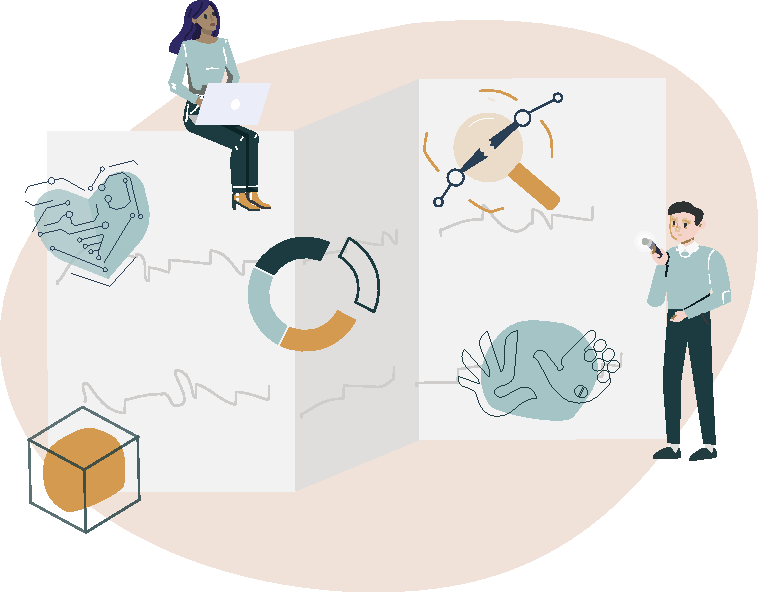
\includegraphics[keepaspectratio,alt={Os cinco princípios da ética da IA}]{img/big-five.pdf}}
\caption{Os cinco princípios da ética da IA}
\end{figure}

Os cinco princípios da ética da IA respondem a perguntas diferentes e se
concentram em valores diferentes:

\begin{enumerate}
\def\labelenumi{\arabic{enumi}.}
\tightlist
\item
  Devemos usar a IA para o bem e não para causar dano? (princípio da
  beneficência / não-maleficência)
\item
  Quem deve ser responsabilizado quando a IA causa dano? (princípio da
  responsabilização)
\item
  Devemos compreender o que a IA faz e por que faz? (princípio da
  transparência)
\item
  A IA deve ser justa ou não discriminatória? (princípio da equidade)
\item
  A IA deve respeitar e promover os direitos humanos? (princípio do
  respeito aos direitos humanos básicos)
\end{enumerate}

O restante deste curso se concentrará nesses princípios da ética da IA.
Analisaremos o que esses conceitos implicam e como podem ser
interpretados, ao modo da filosofia tradicional: análise conceitual.
Também veremos como esses conceitos vêm sendo aplicados na prática,
discutiremos seus problemas e mencionaremos algumas questões em aberto a
respeito deles.

Na última parte do curso, olharemos para o projeto da ética da IA como
um todo. Faremos a pergunta \emph{cui bono}: a ética da IA é para quem,
e quem ou o que fica de fora?

Por fim, queremos observar que, quando se fala de IA e implicações
sociais, a ética da IA é a primeira da lista. Mas existem outros quadros
teóricos para examinar códigos éticos de sistemas algorítmicos
orientados a dados. Por exemplo, questões sobre as implicações sociais
da IA aparecem em campos como culturas algorítmicas, estudos de gênero e
estudos de mídia, entre muitos outros. Da mesma forma, os aspectos
cognitivos e psicológicos da interação humano-máquina moldam a questão
do arcabouço ético apropriado para a IA. Em suma, há muito mais na ética
da IA do que apenas ética de dados ou de algoritmos.

\begin{reflexao}[Exercícios desta seção]

O material original traz aqui um questionário interativo sobre os cinco
princípios da ética da IA apresentados nesta seção, avaliado por revisão
por pares na plataforma Open edX. As perguntas não constam do
repositório de origem --- ficam no banco de dados da plataforma. Redija
o exercício correspondente em
\texttt{exercicios/capitulo01-exercicios.md}.

\end{reflexao}

\subsubsection{Estudo de caso: tradução de imagens e o que ela
reproduz}\label{estudo-de-caso-traduuxe7uxe3o-de-imagens-e-o-que-ela-reproduz}

\begin{caso}[Uma discussão no Twitter]

Imagine que um dia você acabe numa discussão acalorada no Twitter. Ela
começa com o tuíte de um professor universitário (@TuringLives) sobre um
modelo de tradução de imagens. O modelo transformou uma imagem de
entrada pixelada da primeira-ministra finlandesa Sanna Marin na foto de
um homem branco de meia-idade:

\begin{figure}
\centering
\pandocbounded{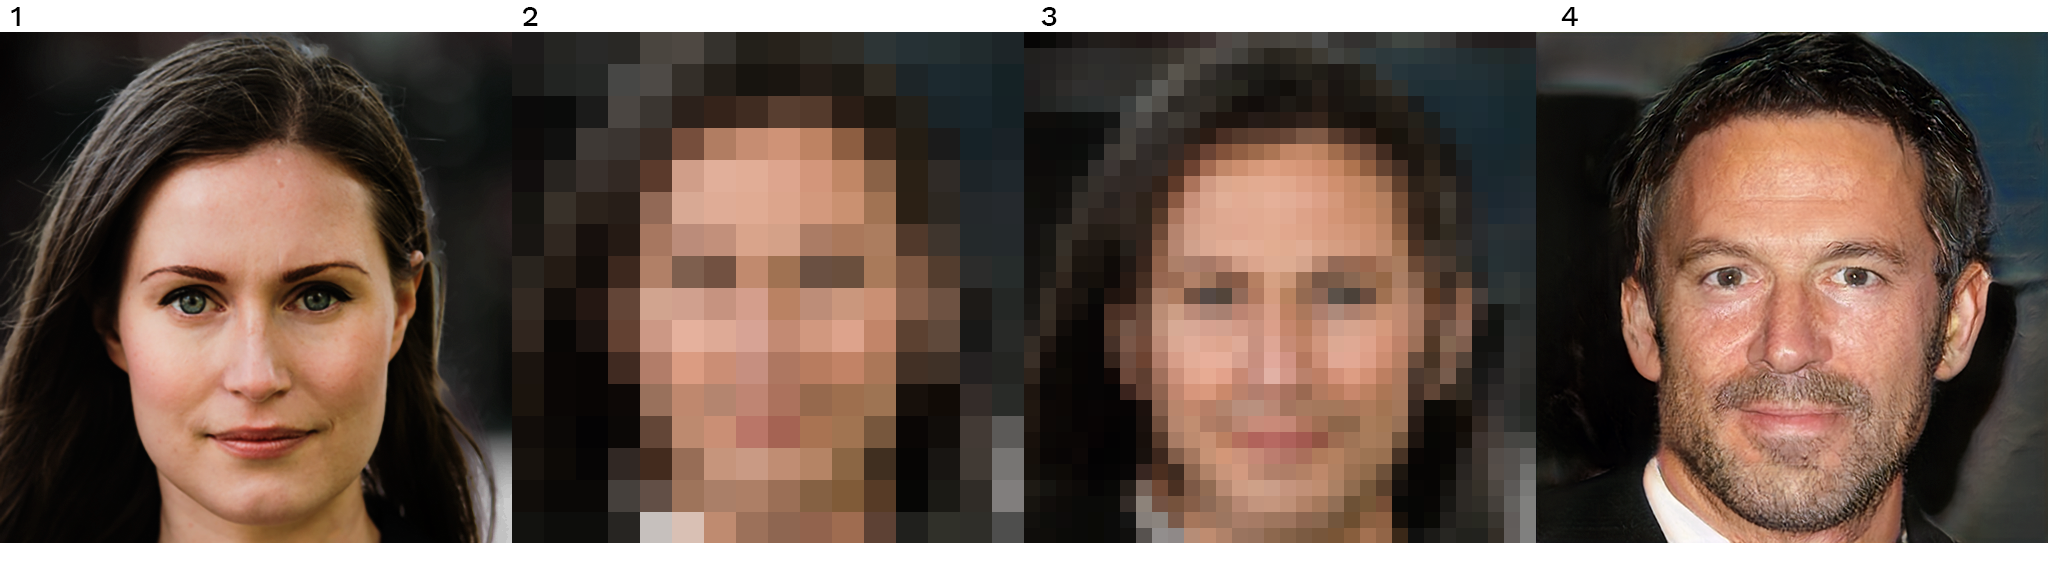
\includegraphics[keepaspectratio,alt={Transformação da imagem de Sanna Marin}]{img/chap1-transf.png}}
\caption{Transformação da imagem de Sanna Marin}
\end{figure}

\textbf{Observação:} este não é um caso real de recriação fotográfica
por IA.

Imagem 1: CC BY 4.0 Laura Kotila / Gabinete da Primeira-Ministra da
Finlândia (editada a partir do original). Imagens 2 e 3 são uma
impressão artística. Imagem 4: CC BY-NC 4.0 NVIDIA Corporation.

\end{caso}

\textbf{O que são algoritmos de tradução de imagens?}

Muitos dos exemplos mais conhecidos de tradução de imagens são
produzidos por uma rede generativa adversarial (\emph{Generative
Adversarial Network}, GAN). Uma GAN é um tipo de arquitetura de rede
neural voltada à modelagem generativa.

Nas GANs, duas redes competem entre si. Uma delas é treinada para gerar,
por exemplo, imagens semelhantes às dos dados de treinamento (gatos,
rostos humanos ou outras coisas). A tarefa da outra rede (chamada rede
adversarial) é separar as imagens geradas pela primeira das imagens
reais dos dados de treinamento.

O sistema treina os dois modelos lado a lado. Na primeira fase do
treinamento, a tarefa do modelo adversarial é distinguir as imagens
reais dos dados de treinamento das tentativas desajeitadas do modelo
generativo. Contudo, à medida que a rede generativa vai lentamente
melhorando, o modelo adversarial também precisa melhorar. O ciclo
continua até que, por fim, as imagens geradas sejam quase
indistinguíveis das reais. (Para mais informações sobre GANs, veja o
curso online \emph{Elements of AI}.)

As GANs não tentam apenas reproduzir os itens dos dados de treinamento.
O sistema é treinado de modo a ter de gerar itens novos e de aparência
real, como imagens. No entanto, as GANs --- como muitos outros
algoritmos contemporâneos --- produzem resultados que refletem os
padrões estatísticos dos dados de entrada.

Essas imagens foram desenvolvidas num projeto de pesquisa de Tero
Karras, Samuli Laine, Timo Aila e Jaakko Lehtinen no NVIDIA Research
Helsinki
(\href{https://research.aalto.fi/en/publications/progressive-growing-of-gans-for-improved-quality-stability-and-va}{veja
este artigo para mais informações}).

\begin{figure}
\centering
\pandocbounded{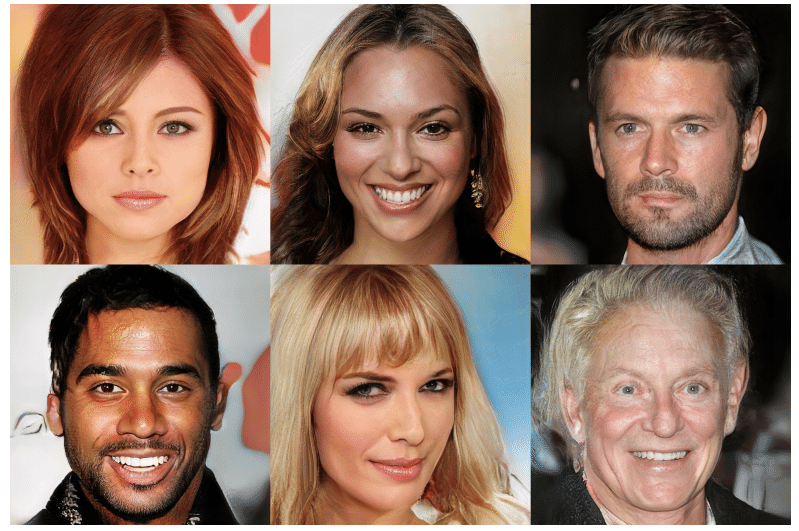
\includegraphics[keepaspectratio,alt={Rostos gerados por GAN}]{img/Exercise_3_image_2.png}}
\caption{Rostos gerados por GAN}
\end{figure}

As GANs podem ser usadas para muitos fins, como tarefas de tradução de
imagem para imagem --- converter fotos de noite em fotos de dia --- ou
gerar fotos fotorrealistas de itens, objetos, cenas ou pessoas.

Para ver como as GANs funcionam, acesse:
http://gandissect.res.ibm.com/ganpaint.html

A seguir, você vai entrar na discussão do Twitter. Sua tarefa é
responder a esses tuítes formulando sua própria opinião sobre o assunto.

\begin{figure}
\centering
\pandocbounded{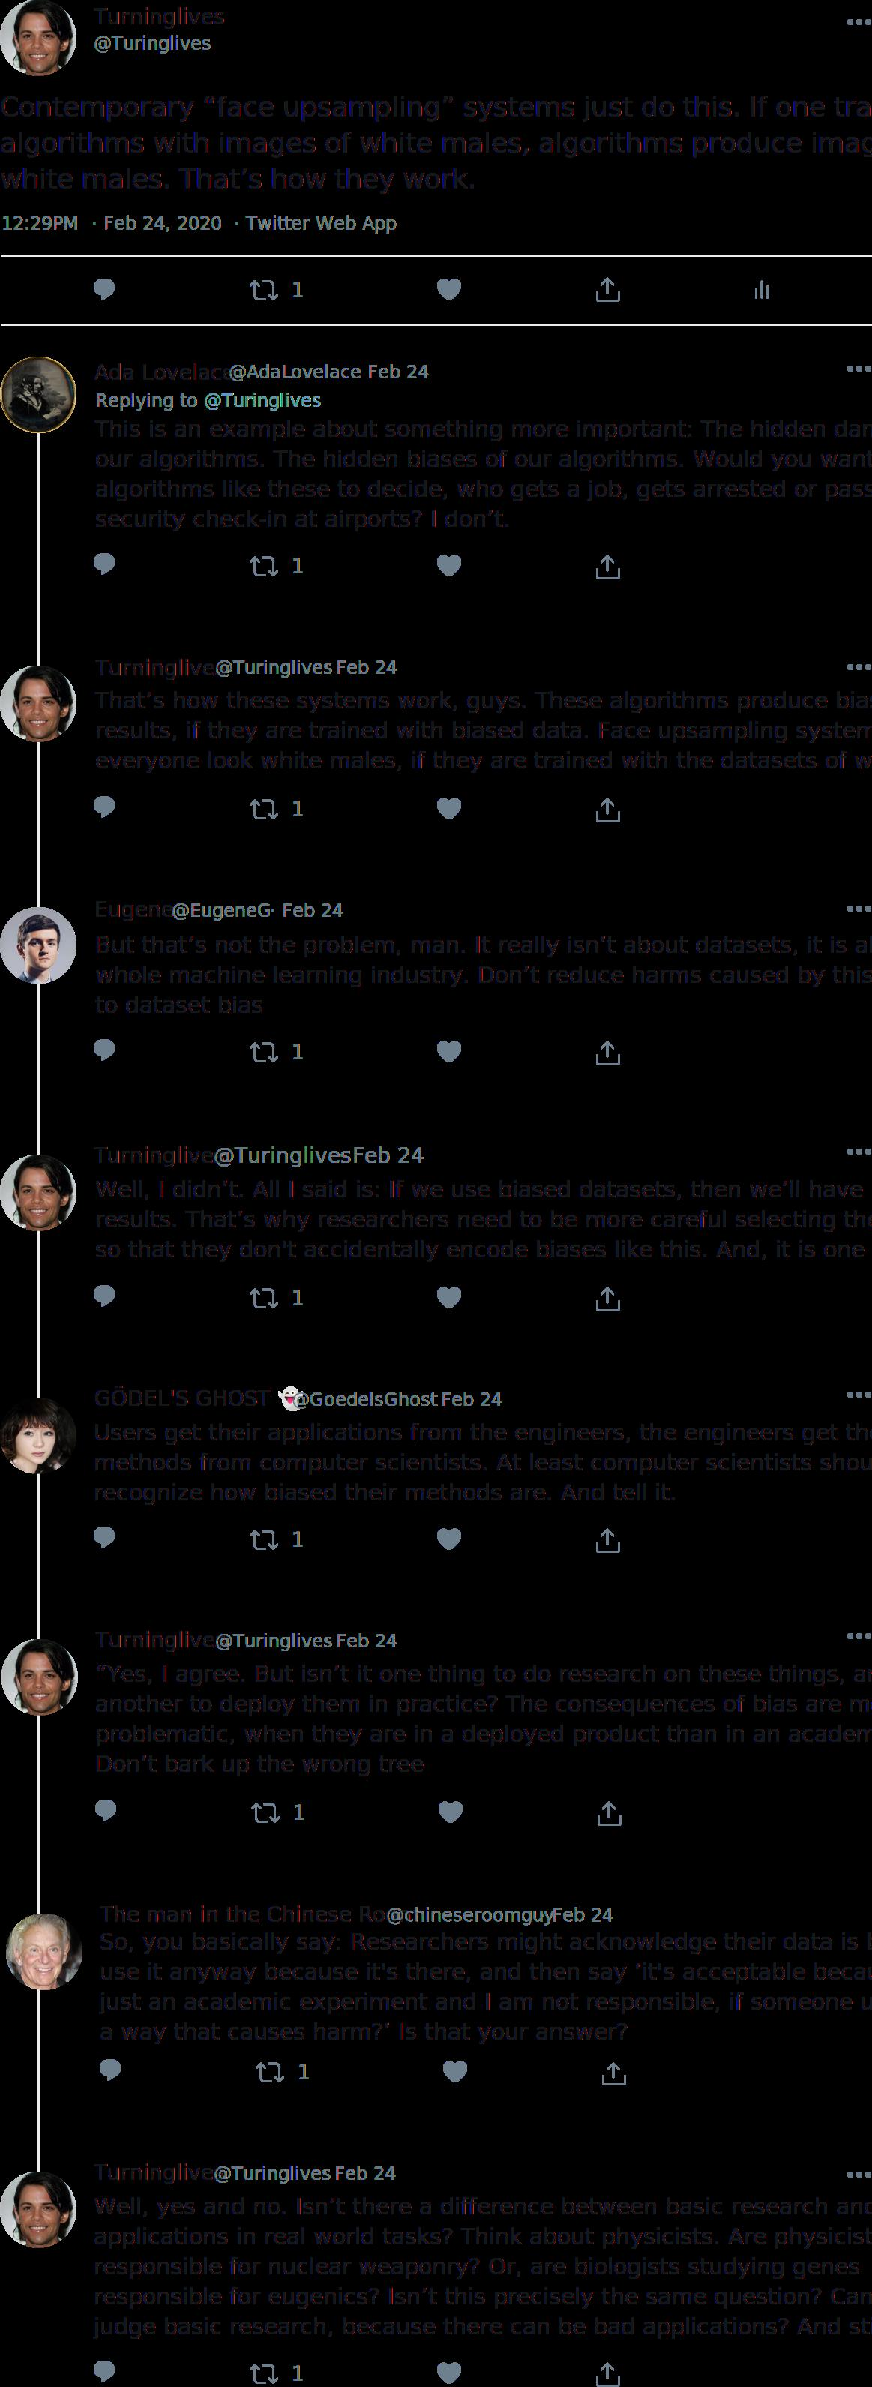
\includegraphics[keepaspectratio,alt={Discussão no Twitter}]{img/twitter-image.pdf}}
\caption{Discussão no Twitter}
\end{figure}

Como você responderia? Desenvolva um nome de usuário no Twitter para si
mesmo e escreva sua resposta abaixo.

\begin{reflexao}[Exercícios desta seção]

No material original, o estudo de caso termina com uma tarefa
dissertativa: entrar na discussão do Twitter, desenvolver um nome de
usuário para si mesmo e responder ao tuíte do professor (@TuringLives)
sobre a transformação da imagem de Sanna Marin, formulando sua própria
posição sobre o assunto. Redija a versão em português desse exercício em
\texttt{exercicios/capitulo01-exercicios.md}.

\end{reflexao}

\subsection{Referências}\label{referuxeancias}

Jobin, A., Ienca, M., \& Vayena, E. (2019). The global landscape of AI
ethics guidelines. \emph{Nature Machine Intelligence}, 1(9), 389--399.

Asimov, I. (1942). Runaround. \emph{Astounding Science Fiction}.

Hume, D. (1739--40). \emph{A Treatise of Human Nature}.

Aristóteles. \emph{Nicomachean Ethics}, 1094a.

Karras, T., Laine, S., Aila, T., \& Lehtinen, J. (2018). Progressive
Growing of GANs for Improved Quality, Stability, and Variation.
\emph{ICLR 2018}.

\begin{center}\rule{0.5\linewidth}{0.5pt}\end{center}

\begin{licenca}

\textbf{Material original:} \emph{Ethics of AI}, um curso online
gratuito da Universidade de Helsinque. Professores responsáveis:
Anna-Mari Rusanen e Jukka K. Nurminen. Demais contribuintes principais:
Santeri Räisänen, Sasu Tarkoma e Saara Halmetoja. Disponível em
\url{https://ethics-of-ai.mooc.fi/}.

\textbf{Esta versão:} tradução e adaptação para o português brasileiro
realizada por José Lucas Lira Bizil, Fernando Mazzeto Lisboa Lima e
Matheus da Silva Fernandes, no âmbito do Programa CiberExt 26-29
(FEELT38103), Universidade Federal de Uberlândia, 2026. Esta é uma obra
derivada; os autores originais não a revisaram nem a endossam.

\textbf{Licença:} Creative Commons
Atribuição-NãoComercial-CompartilhaIgual 4.0 Internacional (CC BY-NC-SA
4.0) ---
\url{https://creativecommons.org/licenses/by-nc-sa/4.0/deed.pt-br}.

\end{licenca}

\end{document}
